% Section Optimisation des terminaux à conteneurs

\subsection*{Introduction}

Le Terminal de Normandie est un exemple de terminal portuaire à conteneurs parmi tant d'autres. 
De façon générale, un terminal multimodal à conteneurs est une plate-forme logistique où les échanges doivent être réalisés dans le respect de certains critères (emplacements de stockage, fenêtres de temps, ressources humaines, etc.). 
Un certain nombre d'éléments peuvent ainsi être optimisés afin de répondre au mieux aux besoins des clients tout en maximisant les profits pour le terminal.

Les terminaux sont en concurrence les uns avec les autres. Les navires choisissent les ports leur permettant de décharger leur cargaison et de charger de nouveaux conteneurs le plus rapidement possible et pour le coût le plus faible possible. Les ports de Rotterdam, de Hambourg, d'Anvers, de Brême et du Havre sont ainsi en concurrence pour desservir le Nord de l'Europe. 
Il est donc primordial pour ces ports de réduire les coûts d'exploitation tout en assurant une productivité élevée.

On retrouve ainsi de nombreux facteurs d'optimisation dans les terminaux à conteneurs comme : 
\begin{itemize}
  \item la structure du terminal ;
  \item l'allocation des berges aux navires ;
  \item l'allocation des grues de quai ;
  \item les plans de chargement des navires ;
  \item le transbordement ;
  \item la gestion des conteneurs vides ;
  \item la gestion des effectifs ;
  \item le routage des véhicules ;
  \item le stockage (allocation des travées et des blocs) ;
  \item les transferts (quai - stockage, stockage - stockage, stockage - terre) ;
  \item l'allocation des engins de manutention.
\end{itemize}
Ces problèmes sont présents dans la littérature en tant que \textit{Berth Allocation Problem}, \textit{Quay Cranes Scheduling Problem}, \textit{Ship Loading Plan Problem}, \textit{Shortest Path Problem}, \textit{Block and Bay Allocation Problem}, \textit{Vehicle Routing Problem} et \textit{Job Scheduling Problem}. %Add quotes

\subsection{Structure du terminal}

La structure du terminal est un élément déterminant concernant la performance des engins de manutention qui s'y déplacent. Disposer de grandes zones de stockage permet d'obtenir une surface de stockage importante. Toutefois, inévitablement certains blocs se retrouveront plus éloignés d'une ou de plusieurs zones de transfert (quais, rails, zones des camions). Un quai éloigné d'une zone de stockage destinée aux transferts sur les camions engendrera des durées de déplacement plus importants mais permettra par exemple de raccourcir la distance vis-à-vis de la zone de stockage destinée aux trains.

De même, les engins de manutention doivent la plupart du temps retourner au dépôt en cas d'inactivité. La position du dépôt est donc essentielle afin de minimiser la distance à parcourir pour se rendre du dépôt aux points de collecte des conteneurs, puis pour revenir du point de livraison vers le dépôt.

Tout est affaire de compromis entre le positionnement des composantes du terminal ainsi qu'entre le choix de ces éléments et de leur quantité. Les plus grands terminaux disposent de quais immenses mais requièrent également par exemple une distance importante entre l'extrémité d'une berge et une zone de stockage même située au centre du terminal. La plupart de ces terminaux géants sont équipés en conséquence et utilisent des portiques dans les zones de stockage et des engins automatiques pour transporter les conteneurs entre les différentes zones.

Le terminal géant de Yangshan (voir Fig. \ref{fig:optTerminaux:shanghaiCT}), situé à Shanghai en Chine est un exemple de ces paradoxes entre la dimension d'un terminal et sa performance. Il est le plus grand terminal au monde à l'heure actuelle. Même si la construction de ce terminal n'est pas encore terminée, ses quais s'étendent déjà sur 6km de long et comportent 60 portiques. Il a été construit sur une île et a été relié à la métropole chinoise par le \textit{Donghai Bridge}, pont de plus de 35km de long. Le paradoxe de ce terminal gigantesque réside dans 3 points. D'une part il est rentre directement en compétition avec les terminaux déjà existant de Shanghai, ensuite le seul point le reliant au continent est un pont dont le trafic ne pourra être trop important, et enfin, sa capacité est telle qu'il ne sera pas utilisé à plein régime avant plusieurs années. Les coûts d'utilisation d'une telle plate-forme seront donc très élevés ce qui rend le terminal peu attractif vis-à-vis des autres terminaux de la 
ville. L'intérêt majeur du terminal réside dans la profondeur de ses quais qui lui confère la possibilité d'accueillir les plus gros porte-conteneurs actuels. Grâce à cette caractéristique et après étude de la structure du terminal et plus particulièrement de son isolement par rapport à la métropole, le terminal de Yangshan apparaît clairement destiné à des opérations de transbordement.


\begin{figure}[ht]
  \begin{center}
    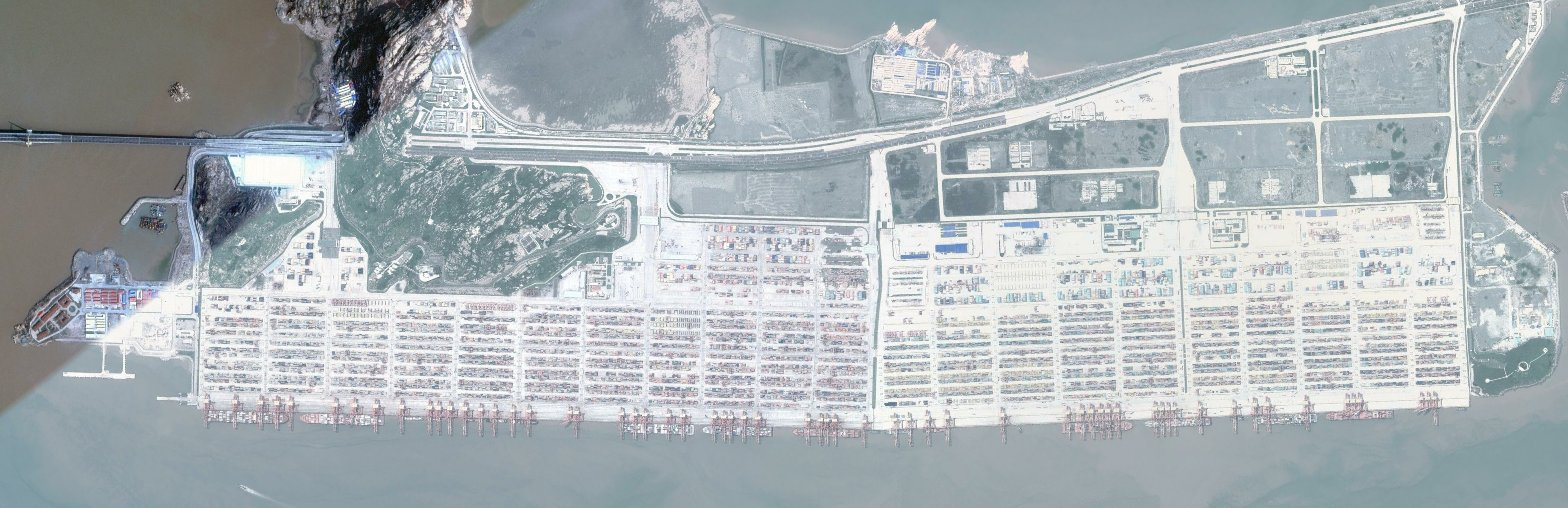
\includegraphics[width=0.8\textwidth]{chapitres/application/terminalDeYangshan.jpg}
    \caption{Terminal de Yangshan à Shanghai en Chine (source : Google Earth)}
    \label{fig:optTerminaux:shanghaiCT}
  \end{center}
\end{figure}

La dimension et l'organisation interne d'un terminal à conteneurs doit donc être étudiée avec le plus grand soin car elle déterminera en grande partie la performance et l'attractivité du terminal.

\subsection{Allocation des berges et transbordement}

Le problème d'affectation des berges (\textit{Berth Allocation Problem} ou \textit{Berth Scheduling Problem}) est l'un des problèmes d'optimisation logistique les plus connus. Il s'agit d'une variante du problème d'affectation quadratique (\textit{Quadratic Assignment Problem}) qui consiste à déterminer l'affectation d'une partie d'un quai à un navire pendant une période donnée de façon à minimiser la durée de service associée au navire (et donc indirectement la distance des déplacements des conteneurs à charger sur le bateau, ou à décharger du bateau, ainsi que les coûts de manutention associés). Tout comme le problème d'affectation quadratique, le problème d'allocation des berges est NP-Difficile.

Ce problème peut se définir dans le cas discret (les quais sont découpés en portions et les navires sont accostés sur un ou plusieurs segments contigus du quai) ou dans le cas continu (le quai n'est pas découpé en parties et les navires peuvent y accoster n'importe où), dans le cas statique (tous les navires sont présents au début du calcul) ou dans le cas dynamique (une partie des navires peuvent être présents au début des calculs, puis les autres arrivent en cours de planification).

Lorsqu'un conteneur doit être déchargé d'un navire pour être chargé sur un autre on parle d'opération de transbordement. Il est alors nécessaire de déterminer conjointement la position d'accostage des deux navires sur le quai afin de minimiser le temps de transfert des conteneurs. 
Lorsqu'un conteneur doit être chargé sur le navire, il faut prendre en compte la distance entre sa position de stockage dans le yard et la position où sera accosté le navire.
Lorsqu'un conteneur doit être déchargé du navire pour être stocké dans le yard, il faut déterminer la position de stockage de ce conteneur en fonction de sa destination future (navire, train ou camion) et chercher un emplacement à la fois proche de la destination et proche du quai où sera accosté le navire. Calculer la position d'accostage du navire revient donc à calculer les emplacements de stockage des conteneurs à décharger de façon à minimiser les déplacements.

%cite

\subsection{Allocation des grues de quai}

Le problème d'affectation des portiques de quai (\textit{Quay Crane Scheduling Problem}) est le problème rencontré une fois le problème de l'affectation du quai résolu, ou du moins en partie résolu. 
En effet, les portiques de quai (\textit{Quay Crane}, \textit{Gantry Crane}, \textit{Container Crane} ou \textit{Ship-to-Shore Crane}) sont des engins de manutention sur rails pouvant mesurer jusqu'à 60 mètres de haut. 
De tels équipements sont extrêmement onéreux et bien souvent les terminaux n'en comportent qu'un nombre restreint. 

Allouer plusieurs portiques au déchargement d'un navire permet de raccourcir la durée de service du navire, mais le portique supplémentaire affecté ne pourra pas être utilisé pour les autre navires accosté au même instant et donc le temps de service des autres navires augmentera.

Les portiques étant posés sur des rails il est impossible de déplacer une grue d'un bout à l'autre du quai si un autre portique se trouve déjà sur le quai. L'affectation d'un portique devra tenir compte de cette caractéristique. 

De même, l'affectation des grues de quai devra également être prise en compte lors de l'affectation de la berge au porte-conteneurs afin de permettre de déterminer son temps de service. 

%cite

\subsection{Positionnement des conteneurs}	%TODO voir avec Monsoria...

Une fois les navires accostés, les portiques affectés au porte-conteneurs se chargent de décharger les conteneurs sur le quai. 
Les conteneurs doivent dans un second temps être acheminés vers un emplacement de stockage en attendant d'être transférés vers un wagon ou un camion ou un autre navire. 
Le choix de cet emplacement doit tenir compte de deux facteurs. D'une part la provenance du conteneur, c'est-à-dire ne pas être situé trop loin du quai dans le cas d'un conteneur déchargé par un portique, ou de la zone du camion ou du train dans le cas d'un conteneur apporté par la route ou par le rail. D'autre part, l'emplacement doit être déterminé en tenant compte de sa destination. Si le conteneur sera chargé sur un wagon alors il devra être stocké dans une travée d'un bloc proche de la zone où le train sera à quai. Si le conteneur sera chargé sur un camion alors d'une part le camion sera dirigé vers une zone d'échange proche du point d'origine du conteneur, et le conteneur sera stocké dans une travée d'un bloc proche de cette zone. Si le conteneur est destiné à être chargé sur un navire, alors il devra être stocké dans la travée d'un bloc à proximité de la portion de quai affectée au navire sur lequel le conteneur devra être chargé.

Il existe également une position verticale à déterminer pour le conteneur. En effet, les conteneurs peuvent être empilés dans les travées sur plusieurs niveaux. Placer un conteneur devant rester dans le terminal longtemps sur le sommet d'une pile alors que les autres conteneurs de cette pile devront être déplacés rapidement engendrera des déplacements supplémentaires. Ces opérations de déplacement consistent un peu comme à la manière du jeu de Hanoï à déplacer temporairement les conteneurs d'une pile sur une autre pile afin de libérer le conteneur posé au sol, puis à reposer les conteneurs supérieurs sur la pile d'origine.
Il est donc important de prendre en compte les fenêtres de temps des missions associées à un conteneur (mission d'entrée du conteneur sur le terminal et mission de sortie du conteneur du terminal) afin de déterminer son emplacement.

Les dates d'entrée et de sortie d'un conteneur sont prises en compte également afin de prioriser l'utilisation d'emplacements proches des zones d'échanges (camions, trains, navires) aux conteneurs transitant peu de temps par le terminal. En revanche, les conteneurs devant rester sur le terminal plus longtemps seront placés plus loin sur les travées de ces zones, ou du moins seront positionnés sur le sol, à la base d'une pile.

Le choix d'un emplacement peut s'avérer difficile si le terminal est saturé. Il peut parfois être nécessaire de déplacer un conteneur à l'intérieur même du yard afin de libérer l'emplacement pour un autre conteneur. Un tel déplacement mobilise un engin de manutention pendant une durée parfois importante et le rend dont inutilisable pour d'autres missions.

Dans le cas statique, où toutes les entrées/sorties de conteneurs sont connues à l'avance, il est possible de déterminer le positionnement optimal des conteneurs afin de minimiser les distances les durées ou de service des clients. En revanche, dans le cas dynamique, les ordres de mission ne sont connues qu'en partie à l'avance, d'autres missions ne seront connues que plus tard, pendant le déroulement de la journée d'exploitation du terminal. Il est dans ce cas impossible de connaître le positionnement optimal des conteneurs de façon exacte. Tout l'enjeu de la résolution de ce problème consiste à déterminer la position optimale des conteneurs à un instant fixé en prennant en compte un facteur de risque lié à la méconnaissance des données.

\subsection{Routage des véhicules} \label{chap:contexte:opt:routageVehicules}

Raccourcir les durées de déplacement entre deux points du terminal permet de réduire le temps de service d'un client. Il est possible d'agir sur 3 facteurs : 
\begin{itemize}
 \item la vitesse de circulation des engins de manutention ;
 \item la limitation de vitesse sur le terminal ; 
 \item le chemin suivi par le véhicule.
\end{itemize}

Le premier facteur dépend des caractéristiques techniques des véhicules, mais touche, comme le second facteur, à la sécurité des personnes et des marchandises sur le terminal. Augmenter la limitation de vitesse d'un engin comme un chariot cavalier demandera aux conducteurs un effort encore plus accru pour maîtriser les 60 tonnes à vide de l'engin et risque de provoquer des accidents aux conséquence lourdes (le conducteur est positionné au sommet de l'engin, soit à plus de 10 mètres du sol).

\begin{figure}[ht]
 \begin{center}
 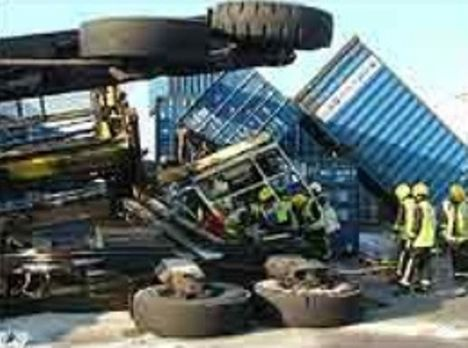
\includegraphics[width=0.4\textwidth]{chapitres/application/sc_crash.jpg}
 \caption{Accident d'un chariot cavalier sur le port d'Essex (Angleterre) le 23 octobre 2007}
 \label{fig:optTerminaux:scCrash}
 \end{center}
\end{figure}

L'unique moyen de chercher à réduire les durées de déplacements au sein du terminal est d'optimiser le guidage des véhicules. 

\subsubsection{Objectifs}
Dans un problème de routage, l'objectif est de minimiser la distance à parcourir entre deux points d'un graphe. 
Comme décrit précédemment, le réseau routier d'un terminal constitue un graphe dont les n\oe{}uds sont les carrefours du terminal et dont les arcs sont les routes et les travées de conteneurs. 

Les chariots cavaliers ont pour objectif d'atteindre des zones de collecte ou de livraisons de conteneurs pendant une fenêtre de temps définie à l'avance. Un routage efficace pour un chariot cavalier consiste donc à atteindre sa destination à l'heure prévue.

Le graphe routier du terminal comporte deux types d'arcs. Si les arcs représentant les routes peuvent facilement absorber un flot de véhicules, les arcs \textit{FIFO} modélisant les travées de conteneurs constituent des points critiques sur le graphe. 
En effet, les chariots cavaliers enjambent les conteneurs empilés dans les travées et ne peuvent donc pas se croiser à l'intérieur de celles-ci. 
Si de tels blocages se produisent ils peuvent causer des retards importants pour la réalisation d'une mission.

Le routage des chariots cavaliers revient à calculer des itinéraires en prenant en compte les temps d'attente en entrée de travées afin de minimiser à la fois la durée totale du parcours (déplacement et attente), le coût de déplacement (consommation de carburant), et l'écart de temps entre la date d'arrivée du chariot et la fenêtre de temps.

\subsubsection{Dynamique du graphe}

Le graphe routier du terminal est donc un graphe partiellement \textit{FIFO} mais ce n'est pas sa seule caractéristique. Ainsi, la durée de parcours d'un arc dépend à la fois de la distance à parcourir (longueur de l'arc) mais également du temps. 

En effet, un chariot cavalier ne se déplace pas à la même vitesse lorsqu'il transporte un conteneur que lorsqu'il se déplace à vide.
Sur le Terminal de Normandie, la vitesse d'un chariot cavalier est de 27km/h à vide contre 23 km/h en charge. 
Il est également à noter qu'un tel véhicule met environ 30 secondes afin d'atteindre les 20 km/h. 
D'autre part la vitesse de circulation d'un chariot cavalier est différente en fonction du type de voie empruntée. 
Ainsi les chariots se déplacent très lentement dans les travées et plus rapidement sur les routes du terminal.

La durée de parcours d'un arc dépend ainsi directement de la vitesse du chariot cavalier, du nombre de décélérations et d'accélérations réalisées, et également du trafic sur l'arc au moment de la traversée.
Les durées d'accélérations et de décélérations se révèlent négligeables en pratique et il est donc possible de simplifier le modèle en ne les prennant pas en compte. La durée de parcours d'un arc $(i,j)$ par un véhicule $v$ au temps $t$ sera représenté par la formule suivante : 

\begin{equation}
 \text{duree(}i,j,v,t\text{)}  = \frac{\text{distance(}i,j\text{)}}{\text{vitesse(}i,j,v,t\text{)}} + \text{attente(}i,j,t\text{)}
 \label{eq:optTerminaux:duree}
\end{equation}

Pour les arcs $(i,j)$ non \textit{FIFO} du graphe, le temps d'attente attente($i,j,t$) sera toujours nul.

\subsubsection{Problème global}

Dans un tel graphe, le problème du plus court chemin en temps peut être résolu en temps polynomial (voir \cite{Orda1990}). 
En revanche, le problème de plus court chemin en coût est NP-difficile (voir \cite{Ahuja2003}). 

Toutefois ce problème devant être résolu pour chaque véhicule du terminal, les résultats du routage d'un véhicule auront un impact sur les caractéristiques du graphe et donc sur le calcul du routage des autres véhicules. 
La résolution globale du problème de routage, c'est-à-dire pour tous les véhicules, repose sur l'ensemble des routages de chaque véhicule (routages locaux). 
Ainsi, lorsqu'un itinéraire est affecté à un chariot cavalier, il est nécessaire de vérifier si une légère modification d'une route déjà établie pour un autre véhicule n'améliorerait pas de façon significative la solution globale. 
Pour trouver la solution globale optimale, il faudrait alors calculer toutes les permutations possibles des solutions locales. 
Ce problème global est donc NP-complet.

\subsection{Ordonnancement et affectation des missions}

L'ordonnancement des missions consiste à déterminer une date d'exécution à chaque mission ainsi qu'à leur affecter une ressource, c'est-à-dire un chariot cavalier. 

%\subsubsection{Deux problèmes dépendants} 

La date d'exécution de la mission dépendra de deux facteurs. D'une part la fenêtre de temps associé à la phase de collecte du conteneur, et d'autre part la position du chariot cavalier affecté à la mission. En effet, la durée du déplacement du véhicule de sa position initiale à l'emplacement de collecte du conteneur sera prise en compte afin de déterminer la date d'exécution de la mission.

D'autre part, le choix du véhicule affecté à la mission dépendra de 2 facteurs. 
Tout d'abord, la compatibilité du véhicule avec la mission. En effet, certains chariots cavaliers ne sont pas capable d'adapter la taille de leur \textit{spreader} sans devoir être modifié au dépôt par un mécanicien. C'est pourquoi, en fonction du type de conteneur à déplacer il sera impossible pour certains véhicules de remplir la mission, ou la date d'exécution de la mission devra prendre en compte la durée de déplacement du chariot vers le dépôt ainsi que la durée de la modification par le mécanicien.
Ensuite, le deuxième facteur de choix du véhicule pour une mission particulière correspond à son activité, c'est-à-dire à son plan de charge au moment de l'ordonnancement. C'est en effet son activité qui déterminera sa position au moment de l'exécution ainsi que sa future destination après avoir accompli la mission planifiée.
L'objectif est de choisir le véhicule dont l'insertion de la mission dans le plan de charge fera le moins augmenter la distance totale parcourue par l'ensemble de la flotte de véhicules, tout en respectant les contraintes temporelles.

Il est clair que le calcul de la date d'exécution de la mission dépend du chariot qui lui a été affecté et que le choix du chariot est fonction de la date d'exécution de la mission. Le calcul des dates d'exécution et l'affectation des missions aux véhicules doivent donc faire partie du même processus de calcul.\\

Ce problème fait l'objet de cette thèse. Nous détaillerons ainsi dans le chapitre suivant, les différentes modélisations du problème ainsi que la méthode de résolution que nous avons élaboré permettant de proposer des solutions de façon dynamique.
